\documentclass[zihao=false,fontset=windows]{ctexart}
% ctexart 不接受任意 pt 选项。正文改 {10pt}，方括号里是行距。
\usepackage{scrextend}
\changefontsizes[12pt]{10pt}

\usepackage[a4paper,left=2.35cm,right=2.35cm,top=1.7cm,bottom=1.9cm]{geometry}
\usepackage{xcolor}
\usepackage{graphicx}
\usepackage{amsmath,amssymb}
\usepackage{enumitem}
\usepackage{tabularx}
\usepackage{colortbl}
\usepackage{listings}
\usepackage{hyperref}
\usepackage[most]{tcolorbox}

\definecolor{feishuText}{RGB}{31,35,41}
\definecolor{feishuBlue}{RGB}{36,91,219}
\definecolor{feishuRed}{RGB}{216,57,49}
\definecolor{feishuGray}{RGB}{100,106,115}
\definecolor{feishuGray2}{RGB}{143,149,158}
\definecolor{feishuPinkBg}{RGB}{251,191,188}
\definecolor{quoteBar}{RGB}{51,112,255}
\definecolor{codebg}{RGB}{245,246,247}
\definecolor{codeborder}{RGB}{222,224,227}
\definecolor{inlinebg}{RGB}{242,243,245}
\definecolor{callRed}{RGB}{253,226,226}
\definecolor{callOrange}{RGB}{255,245,235}
\definecolor{callYellow}{RGB}{254,255,240}
\definecolor{callGreen}{RGB}{240,251,239}
\definecolor{callBlue}{RGB}{240,244,255}
\definecolor{callRedSoft}{RGB}{254,241,241}
\definecolor{callSun}{RGB}{255,255,204}
\definecolor{tableHead}{RGB}{242,243,245}
\definecolor{tableRule}{RGB}{222,224,227}
\definecolor{codeText}{RGB}{31,35,41}
\definecolor{codeKeyword}{RGB}{0,0,255}
\definecolor{codeComment}{RGB}{0,128,0}
\definecolor{codeString}{RGB}{163,21,21}

\setmainfont{Times New Roman}
\setCJKmainfont{Microsoft YaHei}[AutoFakeBold=2.2]
\setCJKsansfont{Microsoft YaHei}[AutoFakeBold=2.2]
\setCJKmonofont{Microsoft YaHei}[AutoFakeBold=2.2]
\setmonofont{Consolas}
\newfontfamily\emojifont{Segoe UI Emoji}

\hypersetup{
  colorlinks=true,
  urlcolor=feishuBlue,
  linkcolor=feishuBlue,
  unicode=true,
  pdftitle={NaViT}
}

\setlength{\parindent}{0pt}
\setlength{\parskip}{0.42em}
\setlength{\fboxsep}{1.5pt}
\setlength{\emergencystretch}{3em}
\linespread{1.28}
\color{feishuText}
\arrayrulecolor{tableRule}
\urlstyle{same}

\setlist[enumerate]{label=\textcolor{feishuBlue}{\arabic*.}, leftmargin=1.7em, itemsep=0.22em, topsep=0.28em, parsep=0.08em, partopsep=0pt}
\setlist[itemize,1]{label=\textcolor{feishuBlue}{\textbullet}, leftmargin=1.35em, itemsep=0.18em, topsep=0.25em, parsep=0.06em, partopsep=0pt}
\setlist[itemize,2]{label=\textcolor{feishuBlue}{◦}, leftmargin=1.45em, itemsep=0.12em, topsep=0.15em}
\setlist[itemize,3]{label=\textcolor{feishuBlue}{\rule[0.18em]{0.38em}{0.38em}}, leftmargin=1.55em, itemsep=0.1em, topsep=0.12em}

\newcommand{\feiEmoji}[1]{{\emojifont #1}}
\newcommand{\incode}[1]{\colorbox{inlinebg}{\ttfamily\small #1}}
\newcommand{\bigmath}[1]{%
  \begin{center}\large$\displaystyle #1$\end{center}%
}

\lstset{
  language=Python,
  basicstyle=\ttfamily\footnotesize\color{codeText},
  keywordstyle=\color{codeKeyword},
  commentstyle=\color{codeComment},
  stringstyle=\color{codeString},
  showstringspaces=false,
  breaklines=true,
  columns=fullflexible,
  keepspaces=true,
  tabsize=4,
  upquote=true,
  aboveskip=2pt,
  belowskip=0pt,
  xleftmargin=0pt,
  frame=none
}

\tcbset{
  feishubase/.style 2 args={
    enhanced,
    boxrule=0pt,
    arc=8pt,
    left=10pt,
    right=10pt,
    top=7pt,
    bottom=7pt,
    before skip=6pt,
    after skip=6pt,
    colback=#1,
    colframe=#1,
    before upper={\feiEmoji{#2}\hspace{0.45em}\ignorespaces}
  }
}
\newtcolorbox{feishubox}[2]{feishubase={#1}{#2}, breakable}
\newtcolorbox{feishuboxnb}[2]{feishubase={#1}{#2}}

\newtcolorbox{feishuquote}{
  enhanced,
  breakable,
  boxrule=0pt,
  leftrule=3pt,
  arc=0pt,
  colframe=quoteBar,
  colback=white,
  left=8pt,
  right=2pt,
  top=2pt,
  bottom=2pt,
  before skip=4pt,
  after skip=4pt,
  before upper=\color{feishuGray}
}

\newtcolorbox{feishucode}{
  enhanced,
  breakable,
  colback=codebg,
  colframe=codeborder,
  boxrule=0.6pt,
  arc=6pt,
  left=6pt,
  right=6pt,
  top=5pt,
  bottom=4pt,
  before skip=6pt,
  after skip=6pt
}


% 来源：https://scnajei2ds6y.feishu.cn/wiki/N6PmwVkCcisDJGkC7Ypc1SfInwh
% 飞书正文连续读取至文末，公式按可见KaTeX结构转写并视觉核对。
% fig-05为正常网页截图裁剪；fig-04与fig-01为原文重复的同一幅图。

\begin{document}
{\zihao{1}\bfseries NaViT\par}
\begin{feishubox}{callOrange}{📚}
论文：《Patch n' Pack: NaViT, a Vision Transformer for any Aspect Ratio and Resolution》\par
论文链接：\href{https://arxiv.org/abs/2307.06304}{https://arxiv.org/abs/2307.06304}\par
代码仓库（非官方）：\href{https://github.com/kyegomez/NaViT}{https://github.com/kyegomez/NaViT}\par
\end{feishubox}
\par\vspace{1.0em}\noindent{\zihao{-2}\bfseries \textcolor{feishuBlue}{1.} 背景}\par\vspace{0.28em}
之前的Vision Transformer(ViT)存在两个问题（改进点）：\par
\begin{itemize}
\item 输入ViT的图片需要做缩放(resize)处理，使得图片最终能处理成一个定长的序列表征。
\item ViT本身支持变长序列的modeling，但是需要进行packing提高训练效率。
\end{itemize}
NaViT (Native Resolution ViT) 为了解决上面的问题分别使用了：\par
\begin{itemize}
\item Arbitrary resolutions and aspect ratios：保留原始分辨率和宽高比。
\item Sequence packing during training：将多个图片按原始的分辨率做Patch处理后，然后拼接到一个序列中，来实现对不同分辨率图像可统一处理，\href{https://arxiv.org/abs/2307.06304}{论文}称这种方法为Patch n' Pack。
\end{itemize}
然后最直观的效果就是在相同的计算成本下达到更好的效果：\par
\begin{center}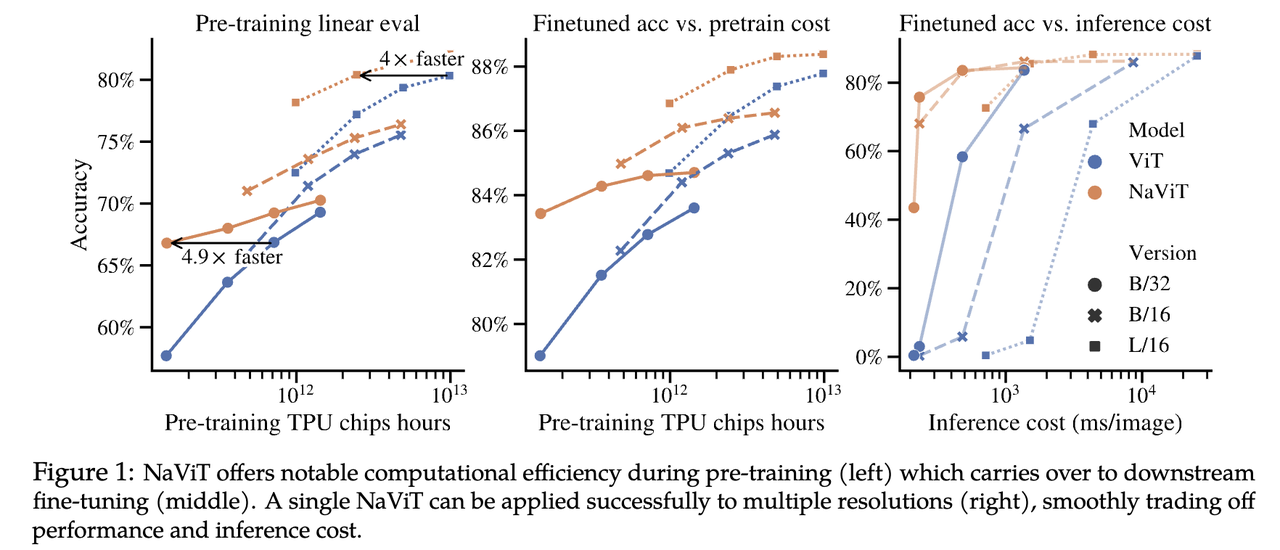
\includegraphics[width=0.98\textwidth]{images/NaViT/fig-01.png}\end{center}
\par\vspace{1.0em}\noindent{\zihao{-2}\bfseries \textcolor{feishuBlue}{2.} NaViT（Native Resolution ViT）}\par\vspace{0.28em}
\par\vspace{1.0em}\noindent{\zihao{3}\bfseries \textcolor{feishuBlue}{2.1} Architectural changes}\par\vspace{0.28em}
\begin{itemize}
\item \textbf{掩码注意力和掩码池化机制} Masked self attention and masked pooling
\end{itemize}
多example打包到一个序列后，在模型前向计算时，Transformer的每一层都会做Self-Attention计算，为了防止不同example相互attention，引入了一个额外的自注意力的掩码。此外通常CV建模任务中，需要对图像所有表征做pooling来计算loss， 同样需要做计算隔离，因此也需要跟Self-Attention计算一样的掩码矩阵。\par
如图所示，一个序列有三个example，token长度分别为: \incode{4,6,5}。最后为了对齐Batch的多序列拼接了\incode{2}个padding token：\par
\begin{center}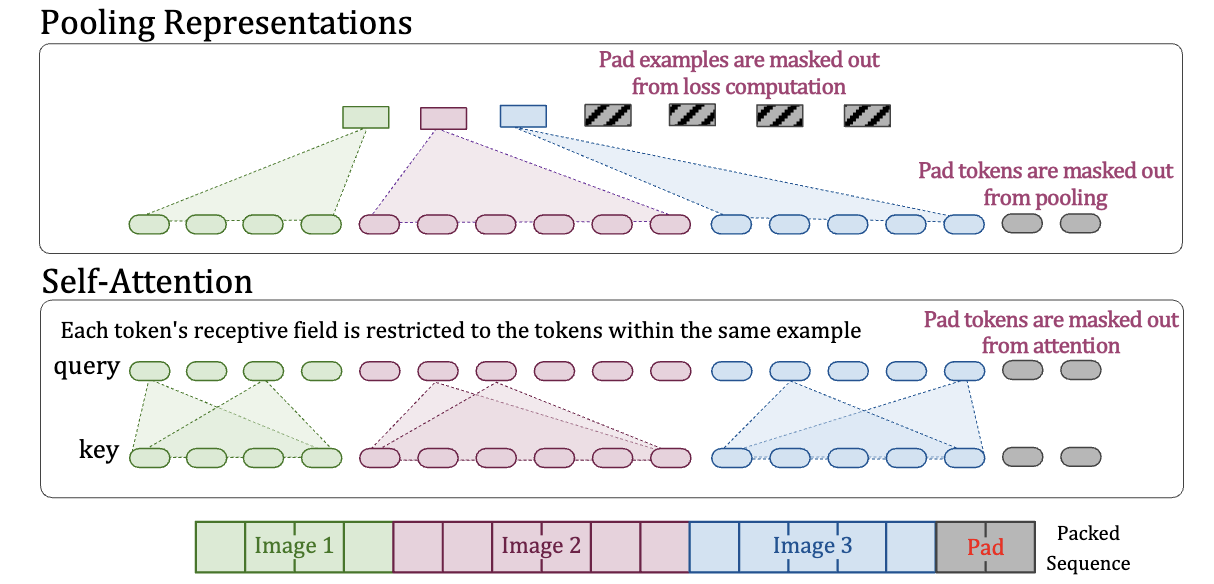
\includegraphics[width=0.98\textwidth]{images/NaViT/fig-02.png}\end{center}
这个额外的Attention Mask其实就是一个对角分块Mask矩阵。\par
\begin{itemize}
\item \textbf{分解\&分数位置编码} Factorized \& fractional positional embeddings
\end{itemize}
（1）ViT用的是一个可训练的1D绝对位置编码。\par
（2）\href{https://arxiv.org/abs/2210.03347}{Pix2struct} 使用的是一个可学习的 2D absolute positional embedding，其大小为 $[\max\_len,\max\_len]$，每个位置 $(x,y)$ 都要被学习过，才能获得较好的效果。\par
（3）NaViT使用的分离式的位置编码对 $x$ 轴和 $y$ 轴的参数分别进行学习，一方面参数量大大减少，由 $\max Len^{2}$ 减少到 $2\times\operatorname{maxLen}$，另一方面分离式的位置编码，对未见过的分辨率有更好的外推性，因为虽然 $(a,b)$ 组合的分辨率没见过，但高是 $a$ 或宽是 $b$ 的图片模型可能分别都见过，这就能学到对应的位置表征。\par
\par\vspace{1.0em}\noindent{\zihao{3}\bfseries \textcolor{feishuBlue}{2.2} Training changes}\par\vspace{0.28em}
\begin{itemize}
\item \textbf{Continuous Token dropping}
\end{itemize}
图像本身是低密度的信息载体，对于空间临近的一些像素和Patch会有较相似的信息，因此在模型训练时，可以通过适当的采样，丢弃一些Patch以提高训练吞吐和性能。\par
对于传统的ViT方法对每个固定分辨率图片只能采用固定drop rate来采样，将每个图片处理成定长的序列以输入给模型。NaViT由于多个image被pack到一个序列里，每个图片可以有不同的drop token的策略，这为不同分辨率的图片提供了灵活的token采样方式，尤其对于一些大尺寸的图片，通过提升drop rate来压缩序列特征长度；同时为了控制Sequence的总长度，可以对最后一个图片做特化的采样策略（如：根据剩余可容纳几个token位置，来设置采样策略），来控制多image拼接后得到一个固定sequence长度，这大大简化了Batch的处理逻辑。\par
\begin{center}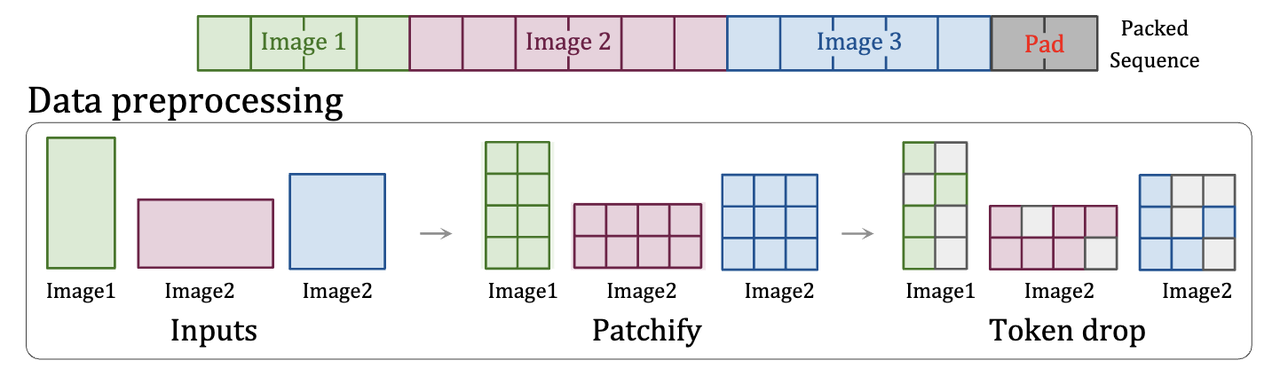
\includegraphics[width=0.98\textwidth]{images/NaViT/fig-03.png}\end{center}
不同图片的预处理过程如图所示，对多图片保留真实的分辨率和宽高比做Patch分块处理，然后对每个图片做不同的drop Token处理，最后拼接成一个序列。\par
\begin{itemize}
\item \textbf{Resolution sampling}
\end{itemize}
NaViT 可以在保持纵横比的同时对图像的像素总数重新采样。\par
对于传统的 ViT 而言，始终存在这样一种权衡：\textbf{使用较小图像训练可以获得更高的吞吐量}（即更快训练），但\textbf{使用较大图像训练则在推断阶段拥有更高分辨率}，因而可能带来更好的模型性能。因此，通常会先以较小分辨率进行预训练，然后在较高分辨率下进行微调。\par
而 NaViT 具有更高的灵活性：它允许对图像尺寸进行混合分辨率采样，同时仍保留每张图像的原始纵横比。这样一来，就能兼顾更高的吞吐量与对大尺寸图像的训练，从而在相同的模型规模与相同的训练时长下，显著提升相对于传统 ViT 的性能。\par
\begin{itemize}
\item \textbf{Padding examples}
\end{itemize}
通过Pack后的序列再组Batch，一个Batch中每个序列包含的example的数量是不同的。NaViT 做了Batch内example对齐处理：\par
对于一个Batch为 $B$ 的序列，我们最多提取 $B\times E_{\max}$ 个pooling后的表征，也就是每个序列都提取 $E_{\max}$ 个图像Pooling的表征。如果一个序列包括超过 $E_{\max}$ 的图像，超过的部分直接丢弃；如果一个序列的examples少于 $E_{\max}$ ，使用 fake 表征对序列做padding。\par
\par\vspace{1.0em}\noindent{\zihao{-2}\bfseries \textcolor{feishuBlue}{3.} Experiments}\par\vspace{0.28em}
与传统的ViT相对，达到传统ViT的最佳性能，只需要更少的计算开销；另外如果使用相同的计算资源，NaViT的性能始终优于ViT。\par
\begin{center}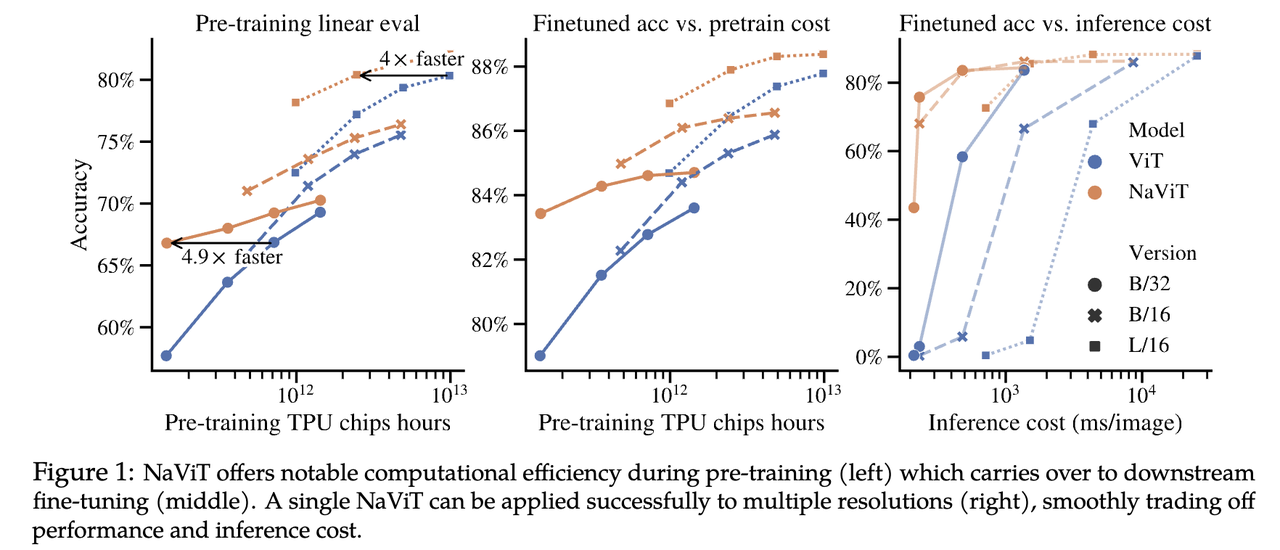
\includegraphics[width=0.98\textwidth]{images/NaViT/fig-04.png}\end{center}
\begin{center}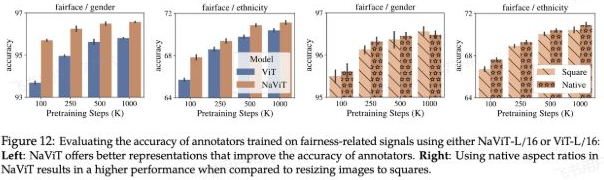
\includegraphics[width=0.98\textwidth]{images/NaViT/fig-05.png}\end{center}
\end{document}